% % % % % % % % % % % % % % % % % % % % % % % % % % % % % % % % % % % % % % % % % % % %
%                                                                                     %
% Short Sectioned Assignment LaTeX Template Version 1.0 (5/5/12)                      %
% This template has been downloaded from: http://www.LaTeXTemplates.com               %
%                                                                                     %
% Original author:  Frits Wenneker (http://www.howtotex.com)                          %
%                                                                                     %
% Modified by: Fco Javier Sueza Rodríguez (fcosueza@disroot.org)                      %
%                                                                                     %
% Changes:                                                                            %
%	    - Custom Chapters, Sections and Subsections (titlesec package)                %
%           - Document type scrbook (oneside)                                         %
%           - Use babel-lang-spanish package and marvosym                             %
%           - Use hyperref, enumitem, tcolorbox and glossaries packages               %
%           - Use Time New Roman (mathptmx), Helvetic and Courier fonts               %
%                                                                                     %
% License: CC BY-NC-SA 3.0 (http://creativecommons.org/licenses/by-nc-sa/3.0/)        %
%                                                                                     %
% % % % % % % % % % % % % % % % % % % % % % % % % % % % % % % % % % % % % % % % % % % %

%-----------------------------------------------%
%	              Packages                  %
%-----------------------------------------------%

\documentclass[paper=a4, fontsize=11pt, oneside]{scrbook}

% ---- Text Input/Output ----- %

\usepackage[T1]{fontenc}
\usepackage[utf8]{inputenc}
\usepackage{mathptmx}
\usepackage[scaled=.92]{helvet}
\usepackage{courier}
\usepackage[indent=12pt]{parskip}

\usepackage{geometry}
\geometry{verbose,tmargin=3cm,bmargin=3cm,lmargin=2.6cm,rmargin=2.6cm}

% ---- Language ----- %

\usepackage[spanish]{babel}
\usepackage{marvosym}

% ---- Another packages ---- %

\usepackage{amsmath,amsfonts,amsthm}
\usepackage{graphics,graphicx}
\usepackage{titlesec}
\usepackage{fancyhdr}
\usepackage{tcolorbox}
\usepackage{hyperref}
\usepackage{enumitem}
\usepackage[automake]{glossaries}

%--------------------------------------------------------------------%
%                      Customizing Document                          %
%--------------------------------------------------------------------%


% ----------- Custom Chapters, Sections and Subsections -------------- %

\titleformat{\chapter}[display]
			{\bfseries\Huge}
			{Tema \ \thechapter} {0.5ex}
			{\vspace{1ex}\centering}

\titleformat{\section}[hang]
			{\bfseries\Large}
			{\thesection}{0.5em}{}

\titleformat{\subsection}[hang]
			{\bfseries\large}
			{\thesubsection}{0.5em}{}

\titleformat{\subsubsection}[hang]
			{\bfseries\large}
			{\thesubsubsection}{0.5em}{}

\hypersetup{
    colorlinks=true,
    linkcolor=black,
    urlcolor=magenta
}

% ------------------- Custom heaaders and footers ------------------- %

\pagestyle{fancyplain}

\fancyhead[]{}
\fancyfoot[L]{}
\fancyfoot[C]{}
\fancyfoot[R]{\thepage}

\renewcommand{\headrulewidth}{0pt} % Remove header underlines
\renewcommand{\footrulewidth}{0pt} % Remove footer underlines

\setlength{\headheight}{13.6pt} % Customize the height of the header

% --------- Numbering equations, figures and tables ----------------- %

\numberwithin{equation}{section} % Number equations within sections
\numberwithin{figure}{section} % Number figures within sections
\numberwithin{table}{section} % Number tables within sections

% ------------------------ New Commands ----------------------------- %

\newcommand{\horrule}[1]{\rule{\linewidth}{#1}} % Create horizontal rule command


%----------------------------------------------------------------------------------------
%	TÍTULO Y DATOS DEL ALUMNO
%----------------------------------------------------------------------------------------

\title{
\vspace{10ex}
\normalfont \normalsize
\huge \textbf{Actividades de la Unidad 3: La Seguridad Social}
}
\author{Francisco Javier Sueza Rodríguez}
\date{\normalsize\today}

%----------------------------------------------------------------------------------------
%                                     DOCUMENTO
%----------------------------------------------------------------------------------------
\begin{document}

\maketitle

\thispagestyle{empty}

\vspace{75ex}

\begin{center}
    \begin{tabular}{l l}
        \textbf{Centro}: & IES Aguadulce \\
        \textbf{Ciclo Formativo}: & Desarrollo Aplicaciones Web (Distancia)\\
        \textbf{Asignatura}: & Formación y Orientación Laboral\\
        \textbf{Tema}: & Tema 3 -  La Seguridad Social\\
    \end{tabular}
\end{center}

\newpage

\tableofcontents

\newpage
\section{Caso Práctico}
Carlos explica a Blanca que como cualquier trabajador en España, debe estar afiliada a la Seguridad Social, es la forma de que participe en el sistema cotizando como trabajadora en activo y de ese modo todos los trabajadores en España, sean del sector que sean y realicen cualquier actividad económica, podamos estar cubiertos, no sólo en asistencia sanitaria, sino también en cuestiones de desempleo y protección.


\section{Actividades}

\subsection{Actividad 1}

\subsubsection{Enunciado}
Una vez trabajada y visto el tema que nos ocupa, te sugiero que elijas una de estas dos opciones:

\begin{enumerate}[label=\alph*)]
    \item Aporta alguna idea o sugerencia personal que consideras que serían convenientes introducir o modificar en la Seguridad Social para mejorar el sistema y justifícala.
    \item Haz una valoración personal sobre la Seguridad Social.
\end{enumerate}

\subsubsection{Solución}
En nuestro caso, hemos elegido la \textbf{opción a} y vamos a aportar alguna idea que sería conveniente introducir en la Seguridad Social.

En mi opinión una buena adición al Sistema de la Seguridad social sería \textbf{ampliar} la \textbf{cobertura dental} que ofrece la Seguridad Social, ya que ahora mismo esta muy limitado, prácticamente cubriendo solo las extracciones dentales y poco más.

Esto se \textbf{justificaría} ya que la salud dental es algo muy importante, ya no solo para la salud de los ciudadanos, sino también para su autoestima, lo que puede influir en sus interacciones sociales, incluida en la búsqueda de empleo. Actualmente, los precios de muchos procedimientos dentales son prohibitivos para familias que tengan poca renta, y aunque algunos pueden considerarse meramente estéticos, otros son necesarios para una buena salud dental, la cual puede afectar a la salud general a varias escalas.

Por ello, la ampliación de la cobertura, por lo menos a los procedimientos relacionados con la salud, como pueden ser endodoncias, empastes, tratamientos de infecciones como la periodontitis, etc.., sería una buena inclusión en la Seguridad Social y tendrían un  impacto muy positivo en muchos ciudadanos.

\subsection{Actividad 2}

\subsubsection{Enunciado}
Contesta las siguientes cuestiones que se plantean:

\begin{enumerate}[label=\alph*)]
    \item Define qué es una contingencia común y ejemplifica.
    \item Define qué es una contingencia profesional y ejemplifica.
    \item Cita los diferentes tipos de prestaciones que nos ofrece la Seguridad Social.
    \item Cita las modalidades de prestaciones de la Seguridad Social y cada modalidad ejemplifícala.
\end{enumerate}

\subsubsection{Solución}

\begin{enumerate}[label=\alph*)]
    \item \textbf{Contingencias Comunes}: son las causadas por alguna enfermedad común o un accidente no laboral,  \textbf{por ejemplo}, una contingencias común sería \textbf{coger alguna enfermedad vírica}, como la Gripe A.

    \item \textbf{Contingencia Profesional}: son aquellas causas por riesgos enfermedad o accidente laboral, \textbf{por ejemplo}, si un operario se \textbf{lesiona una mano} al quedar ésta atrapada en una cinta transportadora.

    \item Las \textbf{principales prestaciones} que nos ofrece la seguridad social son las siguientes:
    \begin{itemize}
        \item Incapacidad Temporal.
        \item Prestación por Nacimiento y Cuidado de Menor.
        \item Suspensión por Riesgo en el Embarazo o Lactancia Natural.
        \item Incapacidad Permanente.
        \item La Jubilación.
        \item Prestación por Muerte y Supervivencia.
        \item Prestación por Desempleo.
    \end{itemize}

    \item La Seguridad Social tiene \textbf{dos modalidades} de prestaciones que son la siguientes:

    \begin{itemize}
        \item \textbf{Prestación Contributiva}: en este tipo de prestaciones no es importante la situación económica del beneficiario, sino que se tienen en cuenta otros requisitos a la hora de poder acceder a ellas, a saber:

        \begin{itemize}
            \item El beneficiario debe estar afiliado a la seguridad social y dado de alta o alta asimilada.
            \item Se deben tener cubiertos los periodos de cotización previos o períodos de carencia, en caso de que sean exigibles, teniendo cada prestación unos límites bien definidos por la ley.
        \end{itemize}

        Este tipo de prestaciones tiene un cuantía económica variables que irá en función de los períodos cotizados y la base reguladora que haya que aplicar dependiendo de la prestación en concreto.

        \textbf{Un ejemplo} de este tipo de prestaciones es \textbf{la jubilación}, donde deberemos de tener una \textbf{cantidad determinada de años cotizados} para poder acceder a ella, y dependiendo de éstos y de la base reguladora que haya que aplicar, los importes a recibir pueden variar enormemente.

        \item \textbf{Prestaciones No Contributivas}: al contrario que en las anteriores, en las prestaciones no contributivas no es necesario tener cubierto un \textbf{período de carencia}, pero si hay están condicionadas a no tener unos ingresos suficientes y a la residencia en el territorio español. La \textbf{cuantía} de este tipo de prestaciones suele ser una cuantía fija para todos los beneficiarios.

        \textbf{Un ejemplo} de estas prestaciones es la \textbf{pensión no contributiva} de \textbf{jubilación}, la cual se concede a trabajadores que no han llegado a cubrir el período de cotización mínimo para acceder a una pensión de jubilación contributiva.
    \end{itemize}
\end{enumerate}

\subsection{Actividad 3}

\subsubsection{Enunciado}
Cumplimenta el siguiente cuadro indicando el régimen  en el que quedan incluidos las personas que aparecen indicadas (puedes marcar con una X). Si en alguno de los ejemplos quieres añadir o comentar algo puedes hacerlo tras el cuadro.

\begin{figure}[H]
    \centering
    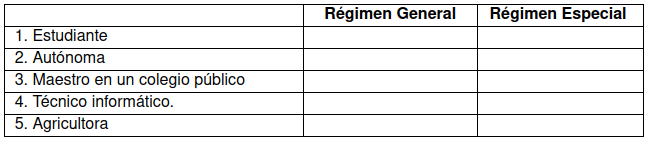
\includegraphics[scale=0.50]{tabla.png}
    \caption{Tabla a rellenar con el régimen de la SS}
\end{figure}

\subsubsection{Solución}

\begin{figure}[ht]

    \vspace{3ex}
    \centering

    \setlength{\tabcolsep}{10pt}
    \renewcommand{\arraystretch}{1.4}

    \begin{tabular}{| l | c | c |}
        \hline
        {} & \textbf{Régimen General} & \textbf{Régimen Especial} \\ \hline
        \centering Estudiante &   & X \\
        \hline
        \centering Autónoma &   & X \\
        \hline
        \centering Maestro de Colegio Público &  X &  \\
        \hline
        \centering Técnico Informático* &  X &  \\
        \hline
        \centering Agricultora &   & X \\
        \hline
    \end{tabular}
\end{figure}

* El técnico informático dependerá de la actividad que desarrolle, se han incluido en el Régimen General, pero si el desarrollara su actividad como autónomo, algo que también es común en la profesión, se incluiría dentro del Régimen Especial, en concreto, dentro del Régimen Especial de Autónomos.

\subsection{Actividad 4}

\subsubsection{Enunciado}
Cita, señala o contesta brevemente:

\begin{enumerate}
    \item Obligaciones formales del empresario con la Seguridad Social.
    \item Sujeto responsable del pago de cuotas (patronal y obrera).
    \item Durante la huelga, ya visto en el tema anterior, ¿Qué sucederá con la obligación económica del pago a la Seguridad Social?
    \item Realiza las capturas de la página web de la Seguridad Social en el que  podemos descargar los modelos referentes al alta y baja de una persona trabajadora.
\end{enumerate}

\subsubsection{Solución}

\begin{enumerate}
    \item Las \textbf{obligaciones formales del empresario} son las siguientes:
    \begin{itemize}
        \item \textbf{Inscripción}: deben inscribir su empresa en la TSGSS.
        \item \textbf{Afiliación}: se trata de la incorporación del trabajador a la Seguridad Social.
        \item \textbf{El Alta}: es el acto de incluir al trabajador en el Régimen General o Especial de la seguridad social.
        \item \textbf{La Baja}: se produce cuando el trabajador cesa el trabajo en su empresa y se tiene que comunicar en los 3 días siguientes.
    \end{itemize}

    \item El \textbf{sujeto responsable} de pagar tanto la cuota patronal como la obrera es el \textbf{empresario}.

    \item Durante \textbf{una huelga}, así como durante un \textbf{cierre patronal}, la obligación económica se \textbf{suspenderá}, siempre y cuando la empresa haya presentado los partes de baja con \textbf{3 días de antelación}. Si no se han presentado los partes de baja, la obligación no se suspenderá.

    \item A continuación se muestra una captura con la página de la Seguridad Social donde se puede descargar el modelo \textbf{TA.2/S}, que es el utilizado tanto para el Alta como la Baja del trabajador, así como para comunicar la variación de datos de este.

    \begin{figure}[H]
        \centering
        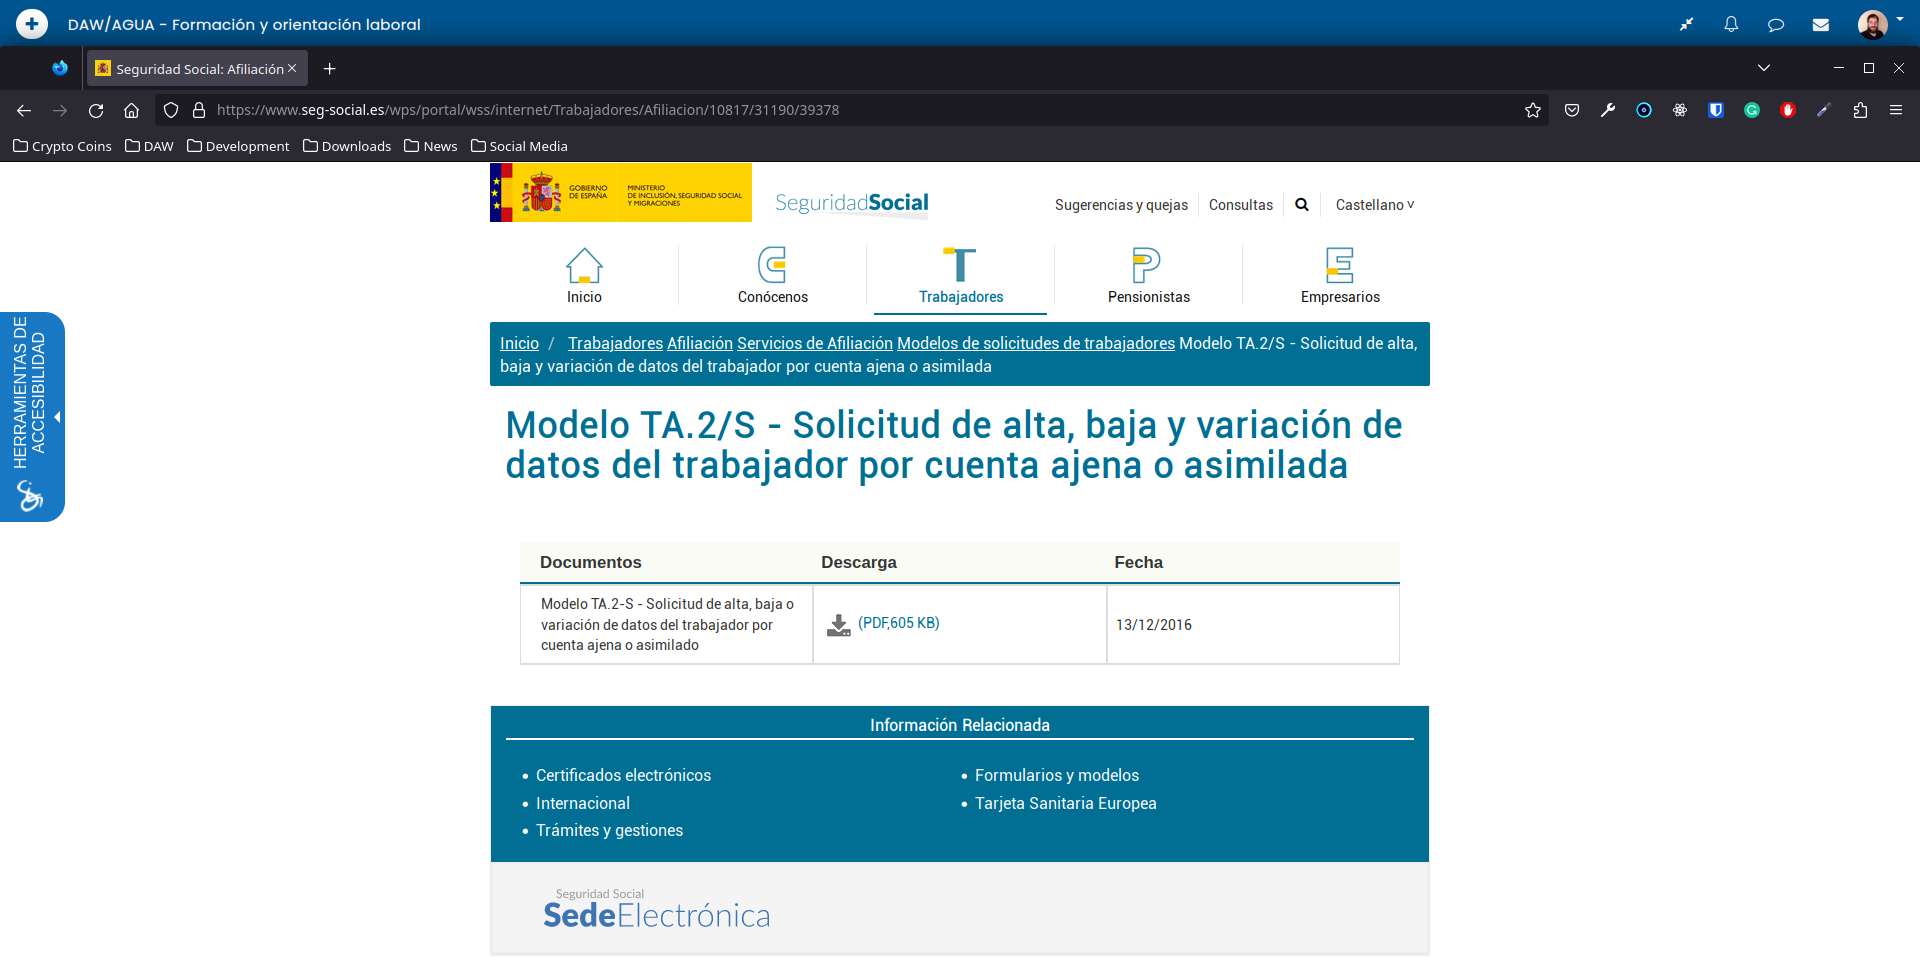
\includegraphics[scale=0.28]{modelo-ts2.png}
        \caption{Descarga modelo TA.2/S en la Web de la SS}
    \end{figure}
\end{enumerate}

\subsection{Actividad 5}

\subsubsection{Enunciado}

Teniendo en cuenta la nómina de la tarea de la unidad anterior (UT01). Determina:

\begin{enumerate}[label=\alph*)]
    \item Las bases de cotización del supuesto explicando cómo se obtienen.
    \item Las cuotas correspondientes al trabajador y el cálculo de las mismas.
    \item La cuotas correspondientes al empresariado y el cálculo de las mismas.
\end{enumerate}

Si en la tarea anterior realizaste la nómina, sólo sería calcular como novedad las deducciones aplicándoles los tipos de cotización (si es que no llegaste a calcularlo). Si tuviste algún error es momento ahora para corregirlo. Si no llegaste a realizarla, ahora puedes hacerlo.

\subsubsection{Solución}
En esta actividad vamos a calcular las diferentes bases de cotización, así como las cuotas correspondientes al trabajador y al empresario. En nuestro caso, ya tenemos prácticamente \textbf{todo calculado} en la \textbf{tarea 1}, por lo que usaremos la información de dicha tarea aunque si explicaremos brevemente como se calcula cada punto.

\begin{enumerate}[label=\alph*)]
    \item En primer lugar vamos a calcular las bases de cotización. Para ello, primero deberíamos haber calculado el \textbf{salario bruto}, sumando todas las retribuciones que recibe el trabajador. En nuestro caso, el s\textbf{salario bruto} calculado es igual a \textbf{1310€}. Una vez calculado el salario bruto, procedemos a calcular cada una de las bases de cotización:

    \begin{itemize}
        \item \textbf{Base de Cotización por Contingencias Comunes}: en este caso, el calculo es similar al del salario bruto, pero no se incluyen las horas extras, en cambio, si se incluyen las pagas \textbf{extras prorrateadas}, obteniendo en nuestro caso una \textbf{base de cotización por contingencias comunes} igual a \textbf{1426,6€}

        \item \textbf{Base de Cotización por Contingencias Profesionales}: en ese caso, solo hay que sumar las horas extras, en el caso de que las hubiera, a la base de cotización por contingencias profesionales, por lo que nosotros hemos obtenido una \textbf{base de cotización por contingencias profesionales} igual a \textbf{1506,6€}
    \end{itemize}

    \item En este punto vamos a calcular las \textbf{cuotas correspondientes al trabajador}. En nuestro caso, ya teníamos calculadas las deducciones, donde se incluían las cuotas del trabajador, solo hay que restar al resultado de las deducciones totales el IRPF, que no forma parte de las cuotas, o obtendremos la cuota del trabajador. En nuestro caso, el \textbf{total de las deducciones} era de \textbf{226,56€}, al que le restamos la proporción del IRPF, esto es, \textbf{131€}.

    Como resultado final, tenemos que la \textbf{cuota del trabajador} es igual a \textbf{95,56€}

    \item Por último, vamos a calcular la \textbf{cuota del empresario}. En este caso hay que volver a calcular las deducciones, pero aplicando los porcentajes pertenecientes al empresario. Así, el calculo ha quedado como vemos en la siguiente tabla:

    \begin{figure}[H]

        \vspace{3ex}
        \centering

        \setlength{\tabcolsep}{10pt}
        \renewcommand{\arraystretch}{1.4}

        \begin{tabular}{| l | r |}
            \hline
            \textbf{Deducción}  & \textbf{Cantidad} \\ \hline
            \centering - Contingencias Comunes (28,30\%) & 336€ \\ \hline
            \centering - FOGASA (0,20\%) & 3€ \\ \hline
            \centering - Desempleo (5,50\%) & 82,8€  \\ \hline
            \centering - FP (0,60\%)& 9€ \\ \hline
            \centering - Horas Extraordinarias (23,60\%) & 18,88€  \\ \hline
            \centering \textbf{TOTAL} &  \textbf{449,68} \\ \hline
        \end{tabular}
        \caption{Cálculo de la cuota empresarial}
    \end{figure}

    Por lo tanto, la \textbf{cuota patronal} para el caso práctico de la Tarea 1 sería de \textbf{449,68€}
\end{enumerate}

\subsection{Actividad 6}

\subsubsection{Enunciado}

\begin{enumerate}[label=\alph*)]
    \item Explica los requisitos básicos y necesarios para poder acceder a una protección contributiva.
    \item Supuesto práctico:

    Todas las personas aquí expuestas creen que tienen derecho a algún tipo de prestación económica de la seguridad social en la modalidad contributiva. Indícales en principio cuál sería y los requisitos para acceder a ella, así como la cuantía, duración y aspectos más relevantes.

    \begin{enumerate}
        \item María José está actualmente embarazada de 7 meses y ya no está en condiciones de trabajar por el ritmo que implica su trabajo. Está  afiliada, dada de alta y trabajando en su empresa desde hace 5 años. Su edad es de 35 años.de baja por maternidad  está afiliada y en alta
        \item Marta, ante la incertidumbre que tiene en su empresa, ha decidido acogerse a una excedencia voluntaria para prepararse unas oposiciones al cuerpo de bomberos.
        \item Ángel, está de baja por una gripe y lleva tres años trabajando en una empresa dado de alta.
        \item Manuel necesita saber para el año 2023 en qué momento nos encontramos del sistema transitorio de pensiones.
    \end{enumerate}
\end{enumerate}

\subsubsection{Solución}
\begin{enumerate}[label=\alph*)]
    \item Para acceder a una \textbf{prestación contributiva}, independientemente de cual sea esta, hay que cumplir dos requisitos básicos. Estos son:
    \begin{enumerate}
        \item Esta \textbf{afiliado} a la Seguridad Social y en situación de \textbf{alta} o \textbf{situación de alta asimilada}.
        \item Tener cubiertos los \textbf{períodos de cotización} previos requeridos en casa caso, también llamados \textbf{períodos de carencia}.
    \end{enumerate}

    \item Para cada uno de los casos expuestos, las prestaciones a las que se pueden acceder son:
    \begin{enumerate}
        \item María podría pedir una \textbf{Suspensión por Riesgo en el Embarazo o Lactancia Natural}. Teniendo en cuenta su caso, la \textbf{duración} de esta prestación sería hasta el \textbf{parto}, o si se diera el caso, a la reincorporación de un \textbf{puesto compatible} con su estado. La \textbf{prestación económica} que recibiría sería del \textbf{100\% de la base reguladora}.

        \item  Marta \textbf{no puede recibir} ningún tipo de prestación de la Seguridad Social, ya que ha cesado de forma voluntaria en su empleo.

        \item Ángel podría acogerse a una prestación de \textbf{Incapacidad Temporal}. En su caso, al ser una \textbf{enfermedad común}, no sería necesario acreditar ningún periodo de carencia. Si esta no fuera una enfermedad común, debería acreditar \textbf{180 días} de cotización en los últimos 5 años, pero al ser una enfermedad común, no es necesario este requisito.

        Respecto a la \textbf{cuantía}, sería de un \textbf{60\% de la base reguladora} desde el 4º día hasta el día 20º. A partir de este día, se cobraría el \textbf{75\% de la base reguladora}.

        \item Actualmente, nos encontramos con la siguiente situación en el sistema transitorio de pensiones:
        \begin{itemize}
            \item Respecto a la \textbf{edad de jubilación}, depende de los años cotizados. Si se acreditan más de \textbf{37 años y 9 meses} cotizados, se puede jubilar a los \textbf{65 años}. Si este no fuera el caso, se deberá jubilar a los \textbf{66 años y 9 meses}.
            \item En lo relativo al \textbf{los años cotizados} para \textbf{calcular la pensión}, en la actualidad se tienen en cuenta los ultimos \textbf{25 años cotizados}.

            \item Para obtener el \textbf{100\% de la pensión}, se necesitarán \textbf{36 años y 6 meses} cotizados.
        \end{itemize}
    \end{enumerate}
\end{enumerate}

\subsection{Actividad 7}

\subsubsection{Enunciado}

En estos supuestos prácticos identifica, justifica y expón las posibles situaciones legales de desempleo.

\begin{enumerate}[label=\alph*)]
    \item Pablo ha sido despedido por la empresa aplicándole un despido disciplinario calificado por el juez como procedente
    \item Silvia estando en periodo de prueba ha renunciado voluntariamente en su nueva empresa pero en la anterior estuvo siete años cotizando.
    \item Miriam empresaria ha rescindido  en periodo de prueba el contrato a Bernabé. Tiene acumulado de paro en los últimos seis años 359 días.
\end{enumerate}

\subsubsection{Solución}
En esta actividad vamos a determinar en cuales de los casos propuestos el trabajador se encuentra en un situación legal de desempleo:

\begin{enumerate}[label=\alph*)]
    \item Pablo \textbf{si se encuentra} en una \textbf{situación legal de desempleo}, ya que los despidos disciplinarios, sean o no procedentes, se considera que dejan al trabajador en una situación legal de desempleo.
    \item Silvia \textbf{no se encuentra} en \textbf{situación legal de desempleo}, ya que a renunciado voluntaria a su empleo, situación que en ningún caso, esta cubierta por la prestación por desempleo.
    \item Bernadé \textbf{si se encuentra} en \textbf{situación legal de desempleo}, ya que la extinción de un contrato en el período de prueba por parte del empleo deja al trabajador en situación legal de desempleo, siempre y cuando hayan transcurrido más de 3 meses desde la extinción de su contrato anterior o si la extinción de dicho contrato se ha producido por causas ajenas a su voluntad.
\end{enumerate}

\subsection{Actividad 8}

\subsubsection{Enunciado}
Oscar se queda en paro en el mes de mayo. Su Base de Cotización de los últimos seis meses ha sido de 1800 € mensuales, y ha cotizado 1240 días en los últimos seis años.

\begin{enumerate}[label=\alph*)]
    \item Calcula la prestación de desempleo a la que tiene derecho y expón el procedimiento seguido para obtenerla.
    \item Haz una captura de la entidad que gestiona dicha prestación.
    \item Cita los requisitos para tener derecho al cobro de la prestación en la modalidad contributiva.
\end{enumerate}

\subsubsection{Solución}
\begin{enumerate}[label=\alph*)]
    \item En primer lugar, vamos a calcular la prestación de desempleo que le corresponde a Óscar.
    \begin{itemize}
        \item \textbf{Duración}: en primer lugar vamos a calcular la duración de la prestación. Óscar tiene acumulados \textbf{1240 días}, si dividimos esta cantidad entre \textbf{365 días}, que son los que tiene un año, nos da un total de \textbf{3 años y 3 meses} de cotización.

        Para calcular la duración, hay que tener en cuenta que el \textbf{primer año}, añade \textbf{4 meses} de duración a la prestación, y a continuación se añaden \textbf{2 meses} por cada \textbf{6 meses cotizados} hasta un máximo de 24 meses. Así, para calcular la duración de la prestación de Óscar hemos usado la siguiente formula:

        \begin{figure}[h]
            \begin{tcolorbox}[sharp corners, colback=yellow!30, colframe=white!20]
                \scriptsize
                \begin{verbatim}


                 4 meses + (2 meses x (24 meses / 6 meses)) = 12 meses
                \end{verbatim}
            \end{tcolorbox}
        \end{figure}

         Hay que mencionar que en la operación anterior se ha dividido 24 meses entre 6 meses, y no 27 meses que son los que le quedaban a Óscar después del primer año. Esto es así porque \textbf{27 entre 6 nos da un resto de 3}, es decir, los últimos \textbf{3 meses no añaden duración al subsidio} ya que no llegan al mínimo de 6 para poder añadir otros 2 meses y por eso no se cuenta.

         En conclusión, Óscar tendría un subsidio con una \textbf{duración de 12 meses}.

         \item \textbf{Cuantía}: ahora, vamos a calcular la cuantía. Según la legislación actual, Óscar cobraría el 70\% de su base reguladora durante los primeros 6 meses y el 60\% de ésta durante los 6 meses restantes.


         Por lo tanto, Óscar \textbf{cobraría 1260€} (70\% de 1800€) durante los \textbf{primeros 6 meses} y \textbf{1080€} (60\% de 1800€) durante los \textbf{6 meses restantes}.
    \end{itemize}

    \item A continuación se muestra una captura de la página del \textbf{SEPE}, que es la entidad gestora de la prestación por desempleo.

    \begin{figure}[H]
        \centering
        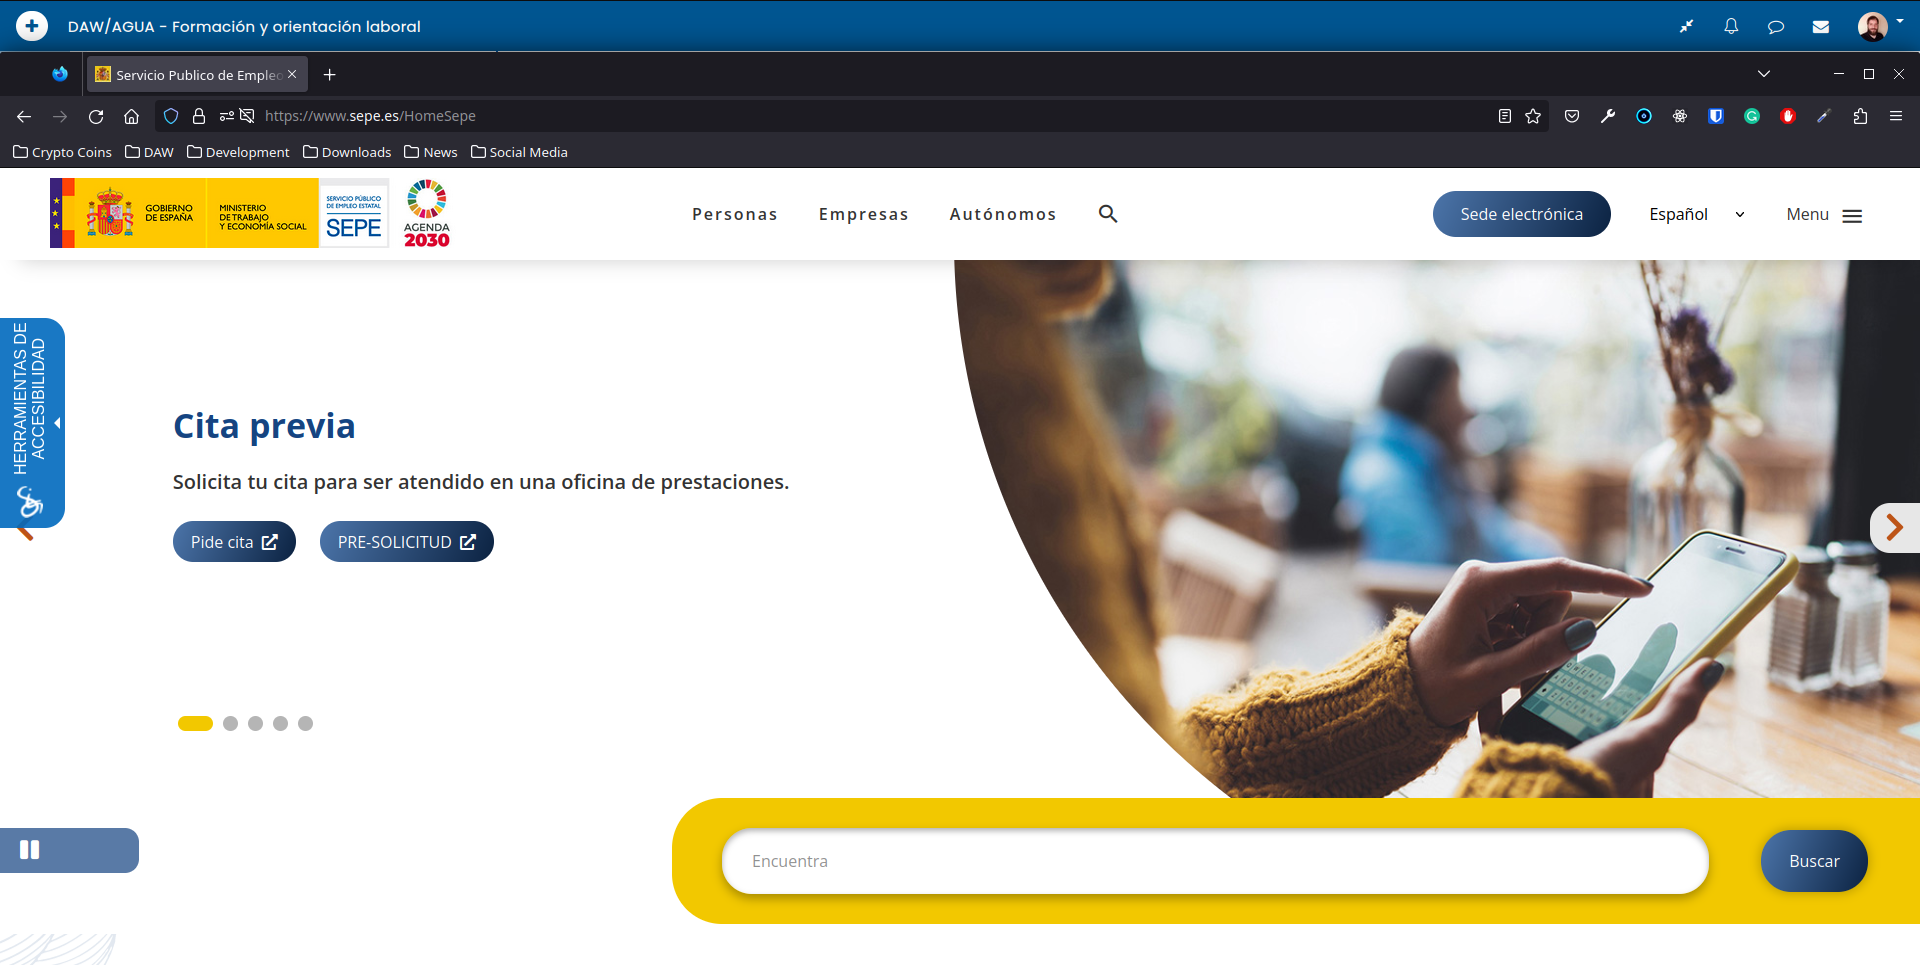
\includegraphics[scale=0.25]{sepe.png}
        \caption{Página principal del SEPE}
    \end{figure}

    \item Para poder acceder a una \textbf{prestación por desempleo en su modalidad contributiva}, los beneficiarios deben cumplir los siguientes requisitos:
    \begin{itemize}
        \item Hallarse en \textbf{situación legal de desempleo} y estar disponible para buscar activamente empleo. La solicitud incluye un \textbf{compromiso de actividad}.
        \item \textbf{Estar afiliado} a la seguridad social y en situación de \textbf{alta} o \textbf{asimilada al alta}.
        \item Estar inscrito como \textbf{demandante de empleo}.
        \item \textbf{No} haber cumplido la \textbf{edad ordinaria para jubilarse}.
        \item \textbf{No cobrar} una pensión de la Seguridad social incompatible con el trabajo.
        \item Haber \textbf{cotizado} un mínimo de \textbf{360 días} en los \textbf{últimos 6 años}.
    \end{itemize}
\end{enumerate}













% Bibliography

\newpage
\bibliography{citas}
\bibliographystyle{unsrt}

\end{document}